\documentclass[11pt]{article}
\setlength{\textwidth}{430pt}\setlength{\oddsidemargin}{11pt}
\usepackage[bottom=0.9in,top=0.9in]{geometry}
\usepackage[utf8]{inputenc}
\usepackage{amsmath}
\usepackage{amsfonts}
\usepackage{mathtools}
\usepackage{enumerate}
\usepackage{tikz}
\usepackage{algorithm}
\usepackage{algorithmic}
\usepackage{hyperref}
\usepackage{graphicx}
\usepackage{listings}
\usepackage{xcolor}
\usepackage{subcaption}
\usepackage{forest}
\hypersetup{
    colorlinks,
    citecolor=black,
    filecolor=black,
    linkcolor=blue,
    urlcolor=black
}

\definecolor{codegreen}{rgb}{0,0.6,0}
\definecolor{codegray}{rgb}{0.5,0.5,0.5}
\definecolor{codepurple}{rgb}{0.58,0,0.82}
\definecolor{backcolour}{rgb}{0.95,0.95,0.92}

\lstdefinestyle{mystyle}{
    backgroundcolor=\color{backcolour},
    commentstyle=\color{codegreen},
    keywordstyle=\color{magenta},
    numberstyle=\tiny\color{codegray},
    stringstyle=\color{codepurple},
    basicstyle=\ttfamily\footnotesize,
    breakatwhitespace=false,
    breaklines=true,
    captionpos=b,
    keepspaces=true,
    numbers=left,
    numbersep=5pt,
    showspaces=false,
    showstringspaces=false,
    showtabs=false,
    tabsize=2
}

\lstset{style=mystyle}

\title{MATH 603 - Final Assignment}
\author{Aiden Taylor - 30092686}
\date{December 5, 2024}

\forestset{replace/.style={if level=#1{label={[label distance=-2mm]south:\vdots}}{if level>=#1{phantom}{}}}}

\begin{document}
\maketitle \newpage \tableofcontents
\newpage
\section{Problems}
	\begin{enumerate}[1.]
		\item Write a computer program to implement the Fast Fourier Transform (FFT).
	\item Using the FFT, write a computer program to solve numerically
		the initial-value problem (IVP) for the heat equation,
			\begin{equation*}
		\begin{cases}
			u_t = u_{xx} & (t,x) \in [0,T] \times [0,L] \\
			u(0,x) = u_0(x) & x \in [0,L]
		\end{cases}.
			\end{equation*}
	\end{enumerate}
\newpage
\section{Problem 1}
To implement the FFT, we should first revist the Continuous Fourier Transform of some function $f(x)$,
	\begin{equation*}
		F(\omega) = \hat{f}(\omega) = \mathcal{F}\left[f\right](\omega) = \frac{1}{2\pi}\int_{-\infty}^{\infty}{f(x)e^{-i\omega x}dx},
	\end{equation*}
where the function can be recovered as
	\begin{equation*}
		f(x) = \int_{-\infty}^{\infty}{\hat{f}(\omega)e^{i\omega x}d\omega}.
	\end{equation*}
Now, consider discretizing both the original and frequency domains into $n$ equally spaced points, where
	\begin{equation}
		\begin{cases}
			\omega_m = 2\pi m/n, & m = 0,1,\dots,n-1, \\
			x_k = x_0 + k\Delta x, & k = 0,1,\dots,n-1,
		\end{cases}
			\label{eq:5}
	\end{equation}
given that $x_0 = 0$ and $\Delta x = L/(n-1)$. Then, if we let $f_k = f(x_k)$ for $k = 0,1,\dots,n-1$,
we can define the Discrete Fourier Transform (DFT) as
	\begin{equation*}
		f_{m}^{\#} = \sum_{k=0}^{n-1}{f_ke^{-i\omega_mk}}, \quad m = 0,1,\dots,n-1,
	\end{equation*}
where the discretization of the function can be recovered as
	\begin{equation*}
		f_{k} = \frac{1}{n}\sum_{m=0}^{n-1}{f_{k}^{\#}e^{i\omega_mk}}, \quad k = 0,1,\dots,n-1,
	\end{equation*}
which we call the Inverse DFT (IDFT). Letting $\xi = e^{i 2\pi/n}$, we can instead represent the DFT and
IDFT respectively as the following two matrix-vector multiplications,
\begin{equation*}
	\begin{bmatrix}
		f_{0}^{\#} \\
		f_{1}^{\#} \\
		f_{2}^{\#} \\
		\vdots \\
		f_{n-1}^{\#}
	\end{bmatrix}
	=
	\begin{bmatrix}
		1 & 1 & 1 & \dots & 1 \\
		1 & \xi^{-1} & \xi^{-2} & \dots & \xi^{-(n-1)} \\
		1 & \xi^{-2} & \xi^{-4} & \dots & \xi^{-2(n-1)} \\
		\vdots & \vdots & \vdots & \vdots & \vdots \\
		1 & \xi^{-(n-1)} & \xi^{-2(n-1)} & \dots & \xi^{-(n-1)(n-1)} 
	\end{bmatrix}
	\begin{bmatrix}
		f_{0} \\
		f_{1} \\
		f_{2} \\
		\vdots \\
		f_{n-1}
	\end{bmatrix},
\end{equation*}
\begin{equation*}
	\begin{bmatrix}
		f_{0} \\
		f_{1} \\
		f_{2} \\
		\vdots \\
		f_{n-1}
	\end{bmatrix}
	=
	\frac{1}{n}
	\begin{bmatrix}
		1 & 1 & 1 & \dots & 1 \\
		1 & \xi^{1} & \xi^{2} & \dots & \xi^{(n-1)} \\
		1 & \xi^{2} & \xi^{4} & \dots & \xi^{2(n-1)} \\
		\vdots & \vdots & \vdots & \vdots & \vdots \\
		1 & \xi^{(n-1)} & \xi^{2(n-1)} & \dots & \xi^{(n-1)(n-1)} 
	\end{bmatrix}
	\begin{bmatrix}
		f_{0}^{\#} \\
		f_{1}^{\#} \\
		f_{2}^{\#} \\
		\vdots \\
		f_{n-1}^{\#}
	\end{bmatrix}.
\end{equation*}
Since both the DFT and IDFT are just $n \times n$ systems,
it follows that they both have a computational complexity of $\mathcal{O}(n^2)$.
From here, the FFT is derived from noticing redundancies in the computation of the DFT, specifically,
from noticing that $\xi$ is periodic and that certain powers of $\xi$ are equal. To illustrate this claim,
consider the system of equations generated by the DFT when $n = 4$,
\begin{equation*}
	\begin{cases}
		f_{0}^{\#} &= f_0\xi^0 + f_1\xi^0 + f_2\xi^0 + f_3\xi^0 \\
		f_{1}^{\#} &= f_0\xi^0 + f_1\xi^{-1} + f_2\xi^{-2} + f_3\xi^{-3} \\
		f_{2}^{\#} &= f_0\xi^0 + f_1\xi^{-2} + f_2\xi^{-4} + f_3\xi^{-6} \\
		f_{3}^{\#} &= f_0\xi^0 + f_1\xi^{-3} + f_2\xi^{-6} + f_3\xi^{-9}.
	\end{cases}
\end{equation*}
If we notice that $\xi^0 = \xi^{-4} = 1$, $\xi^{-2} = \xi^{-6} = -1$, $\xi^{-1} = \xi^{-9} = -i$, and $\xi^{-3} = i$,
then we can simplify the above system of equations to,
\begin{equation*}
	\begin{cases}
		f_{0}^{\#} &= (f_0 + f_1) + \xi^0(f_2 + f_3) \\
		f_{1}^{\#} &= (f_0 - f_1) + \xi^{-1}(f_2 - f_3) \\
		f_{2}^{\#} &= (f_0 + f_1) + \xi^{-2}(f_2 + f_3) \\
		f_{3}^{\#} &= (f_0 - f_1) + \xi^{-3}(f_2 - f_3),
	\end{cases}
\end{equation*}
which has reduced the number of computations from 16 multiplications and 12 additions to 4 multiplications
and 12 additions (without doing any caching or precomputing).
This idea can be generalized when $n$ is some positive integer power of 2,
i.e. $n = 2^{\ell}$ where $\ell \in \mathbb{Z}^+$, which instead allows us to represent the DFT as
\begin{equation}
	\label{eq:1}
	f_{m}^{\#} = \sum_{k=0}^{n-1}{f_k\xi^{-mk}} = \sum_{k=0}^{\frac{n}{2}-1}{f_{2k}\xi^{-m(2k)}} + \sum_{k=0}^{\frac{n}{2}-1}{f_{2k + 1}\xi^{-m(2k+1)}},
\end{equation}
for $m = 0,1\dots,n-1$, where we are essentially just breaking up the summation into its even and odd indexed
summations. If we also notice that
\begin{equation}
	\begin{aligned}
		f_{m}^{\#} &= \sum_{k=0}^{\frac{n}{2}-1}{f_{2k}\xi^{-m(2k)}} + \sum_{k=0}^{\frac{n}{2}-1}{f_{2k + 1}\xi^{-m(2k+1)}} \\
		&= \sum_{k=0}^{\frac{n}{2}-1}{f_{2k}\xi^{-2mk}} + \xi^{-m}\sum_{k=0}^{\frac{n}{2}-1}{f_{2k + 1}\xi^{-2mk}} \\
	\end{aligned}
	\label{eq:2}
\end{equation}
for $m = 0,1,\dots,n-1$, then we can use the idea from (\ref{eq:1}) on each of the two individual summations in (\ref{eq:2}).
Continuing to apply this process recursively until each of the individual summations has just one term,
reduces the computational complexity of the DFT from
$\mathcal{O}(n^2)$ to $\mathcal{O}(n\log_2{n})$, giving us the FFT.
This reduction in complexity can be visualized by the corresponding binary tree generated by the recursive process,

\[
\begin{tikzpicture}[level distance=1.5cm,
  level 1/.style={sibling distance=8cm},
  level 2/.style={sibling distance=4cm},
  level 3/.style={sibling distance=2cm},
  level 4/.style={sibling distance=1cm}]

  \node {$cn$}
    child {node {$cn/2$}
      child {node {$cn/4$}
        child {node {$\vdots$}
          child {node {$c$}}
          child {node {$c$}}
        }
        child {node {$\vdots$}
          child {node {$\ldots$}}
          child {node {$\ldots$}}
        }
      }
      child {node {$cn/4$}
        child {node {$\vdots$}
          child {node {$\ldots$}}
          child {node {$\ldots$}}
        }
        child {node {$\vdots$}
          child {node {$\ldots$}}
          child {node {$\ldots$}}
        }
      }
    }
    child {node {$cn/2$}
      child {node {$cn/4$}
        child {node {$\vdots$}
          child {node {$\ldots$}}
          child {node {$\ldots$}}
        }
        child {node {$\vdots$}
          child {node {$\ldots$}}
          child {node {$\ldots$}}
        }
      }
      child {node {$cn/4$}
        child {node {$\vdots$}
          child {node {$\ldots$}}
          child {node {$\ldots$}}
        }
        child {node {$\vdots$}
          child {node {$c$}}
          child {node {$c$}}
        }
      }
    };
\end{tikzpicture}
\]

where the value at each node in the tree represents an order of the number of floating point operations
required to solve that nodes sub-problem, given that $c$ is some arbitrary constant.
The summation of the values of each node at any particular level of the binary tree should equal $cn$,
so, to compute the computational complexity of this recursive process, we just need to compute the height of this
binary tree.
Now, at the $i^{th}$ level of the binary tree, the values of the
individual nodes at said level represent the $cn/2^i$ floating point operations required to solve that nodes specific
sub-problem,
and at the bottom level we know that we should
only need 
\begin{equation}
	cn/2^i = \mathcal{O}(1) = k
	\label{eq:3}
\end{equation}
floating point operations for each node, where $k$ is also some arbitrary constant value.
So, if
we take the logarithm of both sides of (\ref{eq:3}), we get
\begin{equation*}
	\begin{aligned}
		&\log_2{(cn/2^i)} = \log_2{k} \\
		&\Rightarrow\log_2{cn} - \log_2{2^i} = \log_2{k} \\
		&\Rightarrow\log_2{n} + \log_2{c} - i\log_2{2} = \log_2{k} \\
		&\Rightarrow\log_2{n} + \log_2{c} - \log_2{k} = i
	\end{aligned}
\end{equation*}
which implies that the height of the binary tree is $\mathcal{O}(\log_2{n})$.
Then finally, since we're doing $cn$ floating point operations $\mathcal{O}(\log_2{n})$ times,
we get a computational complexity of $\mathcal{O}(n\log_2{n})$.
The following is an algorithm for the FFT which implements the recursive process that reduces the
computational complexity of the DFT:
\begin{algorithm}
\caption{Fast Fourier Transform}
\begin{algorithmic}[1]
	\STATE \textbf{Procedure} \textsc{FFT}($f$, $f^{\#}$, $n$, $\xi$)
        \IF{$n \gets 1$}
	    \STATE $f^{\#}[0] \gets f[0]$
	\ELSE
		\STATE $f_e[k] \gets \text{ empty array of size } \frac{n}{2}$
		\STATE $f_o[k] \gets \text{ empty array of size } \frac{n}{2}$
		\FOR{$k$ from $0$ to $\frac{n}{2} - 1$}
			\STATE $f_e[k] \gets f[2k]$
			\STATE $f_o[k] \gets f[2k+1]$
		\ENDFOR
		\STATE $f_e^{\#}[k] \gets \text{ empty array of size } \frac{n}{2}$
		\STATE $f_o^{\#}[k] \gets \text{ empty array of size } \frac{n}{2}$
		\STATE \textsc{FFT}($f_e$, $f_e^{\#}$, $\frac{n}{2}$, $\xi^2$)
		\STATE \textsc{FFT}($f_o$, $f_o^{\#}$, $\frac{n}{2}$, $\xi^2$)
		\FOR{$k$ from $0$ to $n - 1$}
			\STATE $f[k] \gets f_e^{\#}[k \mod{\frac{n}{2}}] + \xi^k f_o^{\#}[k \mod{\frac{n}{2}}]$
		\ENDFOR
        \ENDIF
    \STATE \textbf{End Procedure}
\end{algorithmic}
\end{algorithm}
\newpage
\section{Problem 2}
Writing out the problem again, our goal is to solve numerically the IVP,
			\[
		\begin{cases}
			u_t = u_{xx} & (t,x) \in [0,T] \times [0,L] \\
			u(0,x) = u_0(x) & x \in [0,L]
		\end{cases}
			\]
using the FFT. However, before we discretize any of the domains,
consider taking the Fourier Transform of the unknown function, $u$, in the spatial domain,
\begin{equation*}
	u(t,x) \xRightarrow[]{\mathcal{F}} \hat{u}(t,\omega),
\end{equation*}
and the Fourier Transforms of $u_t$ and $u_{xx}$ in the spatial domain as well,
\begin{equation}
	u_t \xRightarrow[]{\mathcal{F}} \frac{d}{dt}\hat{u}(t,\omega) \quad \text{ and } \quad u_{xx} \xRightarrow[]{\mathcal{F}} -\omega^2\hat{u}(t,\omega).
	\label{eq:4}
\end{equation}
Then rewriting the heat equation in terms of the identities in (\ref{eq:4}) results in
\begin{equation*}
	\frac{d}{dt}\hat{u}(t,\omega) = -\omega^2\hat{u}(t,\omega),
\end{equation*}
which is just an ordinary differential equation (ODE), specifically a decay equation,
which has the well known solution
\begin{equation*}
	\hat{u}(t,\omega) = \hat{u_0}e^{-\omega^2t},
\end{equation*}
where $\hat{u_0}$ is the Fourier Transform of the intital-value function $u_0$.
Now, to solve this IVP numerically, we use the discretization of the frequency and spatial domains
described in (\ref{eq:5}), which gives us a system of ODEs,
\begin{equation*}
	\begin{bmatrix}
		\frac{d}{dt}\hat{u}(t,\omega_0) \\
		\vdots \\
		\frac{d}{dt}\hat{u}(t,\omega_{n-1})
	\end{bmatrix}
	=
	\begin{bmatrix}
		-\omega_0^2\hat{u}(t,\omega_0) \\
		\vdots \\
		-\omega_{n-1}^2\hat{u}(t,\omega_{n-1})
	\end{bmatrix},
\end{equation*}
which in turn has a system of solutions,
\begin{equation*}
	\begin{bmatrix}
		\hat{u}(t,\omega_0) \\
		\vdots \\
		\hat{u}(t,\omega_{n-1})
	\end{bmatrix}
	=
	\begin{bmatrix}
		\hat{u_0}(t,\omega_0)e^{-\omega_0^2t} \\
		\vdots \\
		\hat{u_0}(t,\omega_{n-1})e^{-\omega_{n-1}^2t} \\
	\end{bmatrix},
\end{equation*}
for each step in time, $t$. This gives us a vector of Fourier coefficients at each time step, $t$, and
performing the Inverse FFT (IFFT) on each of these Fourier coefficient vectors recovers the approximation of the unknown function, $u$,
at each time step, $t$, as desired.
To illustrate this numerical process I wrote a Matlab program that implements the following IVP,
		\[
		\begin{cases}
			u_t = u_{xx} & (t,x) \in [0,100] \times [0,1] \\
			u(0,x) = u_0(x) & x \in [0,1]
		\end{cases}
		\]
where
\begin{equation*}
	u_0 =
	\begin{cases}
		1 & x \in [0.3725,0.6235] \\
		0 & \text{otherwise}
	\end{cases}.
\end{equation*}
Now, discretizing our frequency and spatial domains into $n=256$ equally spaced points
will result in the following three plots generated by the Matlab program, which concludes my final assignment:
\newpage
\begin{figure}[ht]
	\centering
	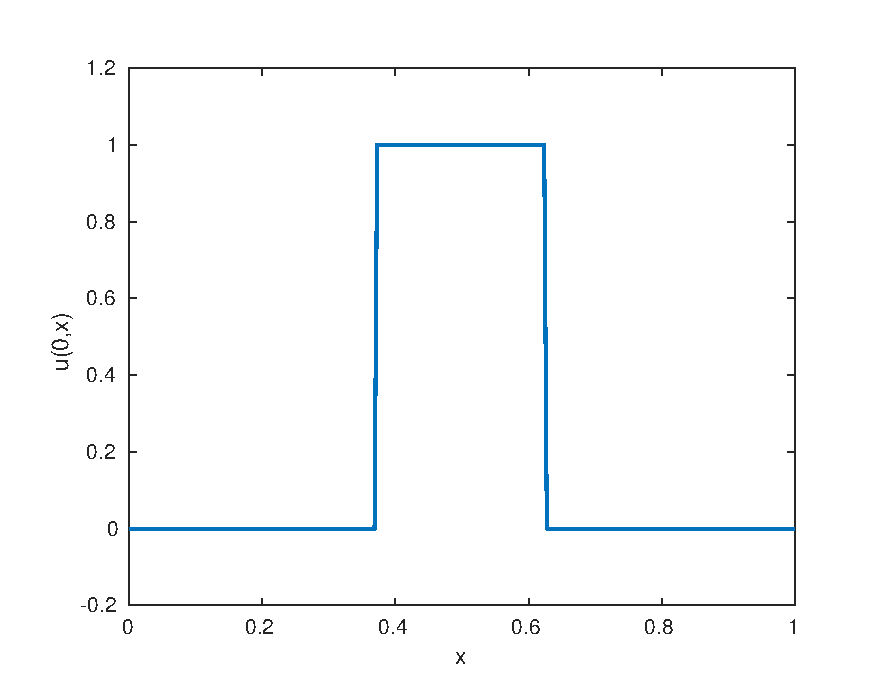
\includegraphics{u0}
	\caption{Plot of $u_0(x)$.}
\end{figure}
\newpage
\begin{figure}[ht]
	\centering
	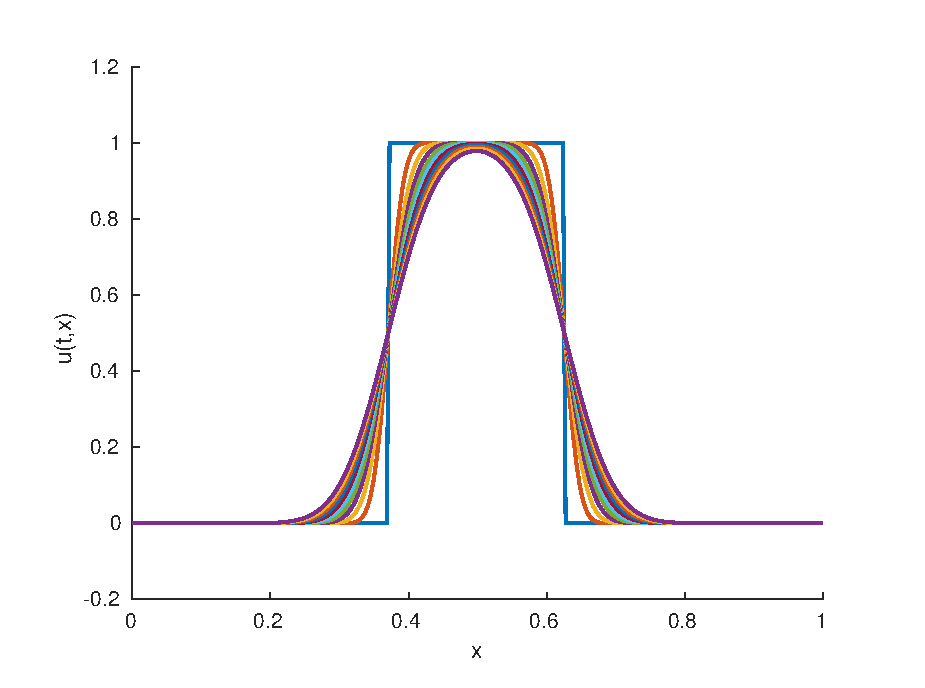
\includegraphics{heat_eq_2d}
	\caption{2-dimensional plot of the numerical solution to the IVP.}
\end{figure}
\newpage
\begin{figure}[ht]
	\centering
	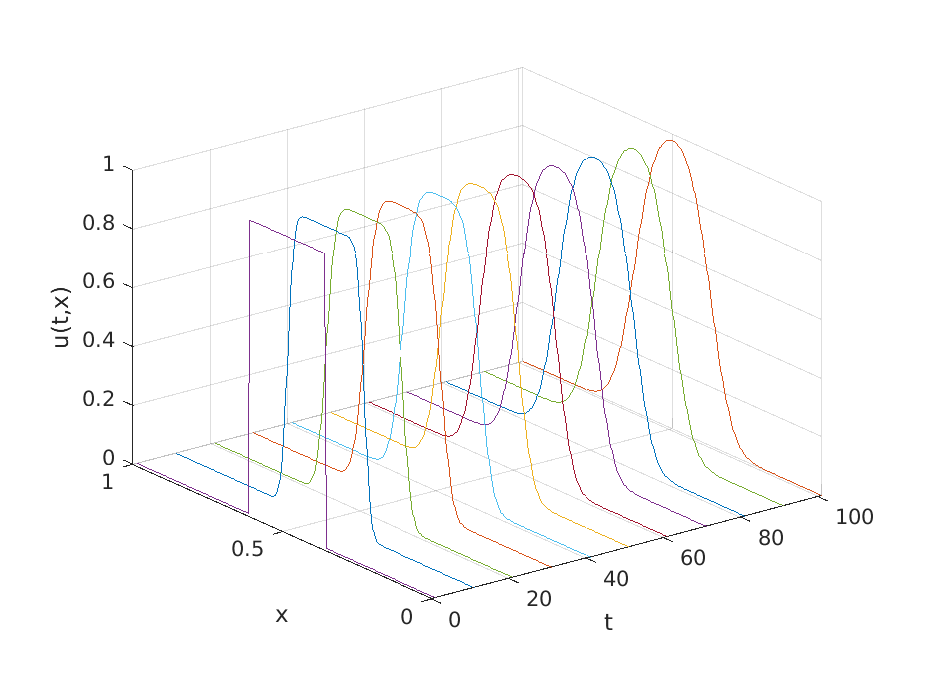
\includegraphics{heat_eq_3d}
	\caption{3-dimensional plot of the numerical solution to the IVP.}
\end{figure}
\end{document}
